\documentclass[12pt,a4paper]{article}

\usepackage[in, plain]{fullpage}
\usepackage{array}
\usepackage{../../../pas-math}
\usepackage{../../../moncours}


%\usepackage{pas-cours}
%-------------------------------------------------------------------------------
%          -Packages nécessaires pour écrire en Français et en UTF8-
%-------------------------------------------------------------------------------
\usepackage[utf8]{inputenc}
\usepackage[frenchb]{babel}
\usepackage[T1]{fontenc}
\usepackage{lmodern}
\usepackage{textcomp}



%-------------------------------------------------------------------------------

%-------------------------------------------------------------------------------
%                          -Outils de mise en forme-
%-------------------------------------------------------------------------------
\usepackage{hyperref}
\hypersetup{pdfstartview=XYZ}
%\usepackage{enumerate}
\usepackage{graphicx}
\usepackage{multicol}
\usepackage{tabularx}
\usepackage{multirow}


\usepackage{anysize} %%pour pouvoir mettre les marges qu'on veut
%\marginsize{2.5cm}{2.5cm}{2.5cm}{2.5cm}

\usepackage{indentfirst} %%pour que les premier paragraphes soient aussi indentés
\usepackage{verbatim}
\usepackage{enumitem}
\usepackage[usenames,dvipsnames,svgnames,table]{xcolor}

\usepackage{variations}

%-------------------------------------------------------------------------------


%-------------------------------------------------------------------------------
%                  -Nécessaires pour écrire des mathématiques-
%-------------------------------------------------------------------------------
\usepackage{amsfonts}
\usepackage{amssymb}
\usepackage{amsmath}
\usepackage{amsthm}
\usepackage{tikz}
\usepackage{xlop}
%-------------------------------------------------------------------------------



%-------------------------------------------------------------------------------


%-------------------------------------------------------------------------------
%                    - Mise en forme avancée
%-------------------------------------------------------------------------------

\usepackage{ifthen}
\usepackage{ifmtarg}


\newcommand{\ifTrue}[2]{\ifthenelse{\equal{#1}{true}}{#2}{$\qquad \qquad$}}

%-------------------------------------------------------------------------------

%-------------------------------------------------------------------------------
%                     -Mise en forme d'exercices-
%-------------------------------------------------------------------------------
%\newtheoremstyle{exostyle}
%{\topsep}% espace avant
%{\topsep}% espace apres
%{}% Police utilisee par le style de thm
%{}% Indentation (vide = aucune, \parindent = indentation paragraphe)
%{\bfseries}% Police du titre de thm
%{.}% Signe de ponctuation apres le titre du thm
%{ }% Espace apres le titre du thm (\newline = linebreak)
%{\thmname{#1}\thmnumber{ #2}\thmnote{. \normalfont{\textit{#3}}}}% composants du titre du thm : \thmname = nom du thm, \thmnumber = numéro du thm, \thmnote = sous-titre du thm

%\theoremstyle{exostyle}
%\newtheorem{exercice}{Exercice}
%
%\newenvironment{questions}{
%\begin{enumerate}[\hspace{12pt}\bfseries\itshape a.]}{\end{enumerate}
%} %mettre un 1 à la place du a si on veut des numéros au lieu de lettres pour les questions 
%-------------------------------------------------------------------------------

%-------------------------------------------------------------------------------
%                    - Mise en forme de tableaux -
%-------------------------------------------------------------------------------

\renewcommand{\arraystretch}{1.7}

\setlength{\tabcolsep}{1.2cm}

%-------------------------------------------------------------------------------



%-------------------------------------------------------------------------------
%                    - Racourcis d'écriture -
%-------------------------------------------------------------------------------

% Angles orientés (couples de vecteurs)
\newcommand{\aopp}[2]{(\vec{#1}, \vec{#2})} %Les deuc vecteurs sont positifs
\newcommand{\aopn}[2]{(\vec{#1}, -\vec{#2})} %Le second vecteur est négatif
\newcommand{\aonp}[2]{(-\vec{#1}, \vec{#2})} %Le premier vecteur est négatif
\newcommand{\aonn}[2]{(-\vec{#1}, -\vec{#2})} %Les deux vecteurs sont négatifs

%Ensembles mathématiques
\newcommand{\naturels}{\mathbb{N}} %Nombres naturels
\newcommand{\relatifs}{\mathbb{Z}} %Nombres relatifs
\newcommand{\rationnels}{\mathbb{Q}} %Nombres rationnels
\newcommand{\reels}{\mathbb{R}} %Nombres réels
\newcommand{\complexes}{\mathbb{C}} %Nombres complexes


%Intégration des parenthèses aux cosinus
\newcommand{\cosP}[1]{\cos\left(#1\right)}
\newcommand{\sinP}[1]{\sin\left(#1\right)}


%Probas stats
\newcommand{\stat}{statistique}
\newcommand{\stats}{statistiques}
%-------------------------------------------------------------------------------

%-------------------------------------------------------------------------------
%                    - Mise en page -
%-------------------------------------------------------------------------------

\newcommand{\twoCol}[1]{\begin{multicols}{2}#1\end{multicols}}


\setenumerate[1]{font=\bfseries,label=\textit{\alph*})}
\setenumerate[2]{font=\bfseries,label=\arabic*)}


%-------------------------------------------------------------------------------
%                    - Elements cours -
%-------------------------------------------------------------------------------





%\makeatletter
%\renewcommand*{\@seccntformat}[1]{\csname the#1\endcsname\hspace{0.1cm}}
%\makeatother


%\author{Olivier FINOT}
\date{}
\title{}

\graphicspath{{./img/}}

\lhead{Seq 3: Fractions}
\rhead{O. FINOT}
%
%\rfoot{Page \thepage}
\begin{document}
%\maketitle




\chap[num=10, color=red]{Proportionnalité}{}

\begin{myobj}
	\begin{itemize}
		
		\item Construire le symétrique d’un point ou d'une figure par rapport à une droite à la main où à l’aide d’un logiciel;
		\item Construire le symétrique d’un point ou d'une figure par rapport à un point, à la main où à l’aide d’un logiciel;
		\item Utiliser les propriétés de la symétrie axiale ou centrale;
		\item Identifier des symétries dans des figures.		
	\end{itemize}
\end{myobj}

\begin{mycomp}
	\begin{itemize}
		\item \kw{Chercher (Ch2)} :  s’engager    dans    une    démarche    scientifique, observer, questionner, manipuler, expérimenter (sur une feuille de papier, avec des objets, à l’aide de logiciels), émettre des hypothèses, chercher des exemples ou des contre-exemples, simplifier ou particulariser une situation, émettre une conjecture ;
		\item \kw{Raisonner (Ra3)} :  démontrer : utiliser un raisonnement logique et des règles établies (propriétés, théorèmes, formules) pour parvenir à une conclusion ;
		\item \kw{Communiquer (Co2)} :  expliquer à l’oral ou à l’écrit (sa démarche, son raisonnement, un calcul, un protocole   de   construction   géométrique, un algorithme), comprendre les explications d’un autre et argumenter dans l’échange ; 
		
	\end{itemize}
\end{mycomp}





\section{Rappel}

\subsection{Grandeurs proportionnelles}

\begin{mydef}
	Deux grandeurs sont \kw{proportionnelles} lorsqu'on peut calculer les valeurs de l'une en multipliant les valeurs de l'autre par un même nombre non nul.
	
	ce nombre est appelé \kw{coefficient de proportionnalité}.
\end{mydef}


\begin{mymeth}
	Pour identifier une situation de proportionnalité, on calcule les quotients des nombres de la seconde ligne par les nombres de la première ligne.
\end{mymeth}

\begin{myex}
	
		On s'intéresse à la distance parcourue à vélo par Aurélie pendant trois jours.
		
		\begin{center}
			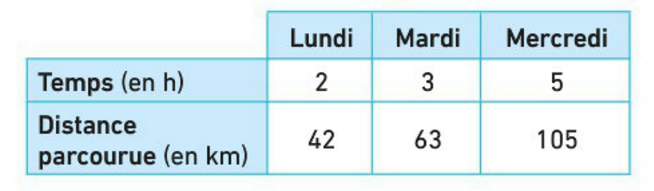
\includegraphics[scale=0.5]{tab1}
		\end{center}
	

	$42 \div 2 = 63 \div 3 = 105 \div 5 = 21$, ici les grandeurs <<temps>> et <<distance parcourue>> sont proportionnelles. Chaque heure elle parcoure 21 km, 21 est le coefficient de proportionnalité.

\end{myex}	

\begin{myex}	
		Dans ce tableau on a reporté le nombre de cotés de certains polygones et leur nombre de diagonales.
		
		\begin{center}
			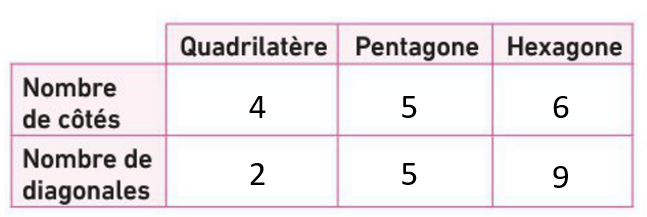
\includegraphics[scale=0.5]{tab2}
		\end{center}
	
		$2 \div 4 = \num{0.5}$, $5 \div 5 = 1$, donc le nombre de côtés d'un polygone n'est pas proportionnel à son nombre de diagonales.	
	
\end{myex}

\subsection{Compléter un tableau de proportionnalité}

\begin{myex}
	On veut remplir le tableau de proportionnalité suivant :
	
	\begin{center}
		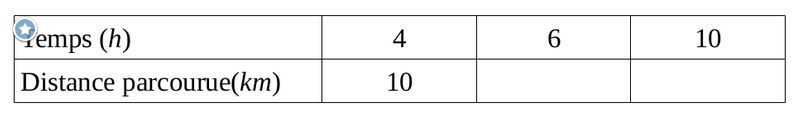
\includegraphics[scale=0.5]{tab3_1}
	\end{center}
\end{myex}


\subsubsection*{Par passage à l'unité}


\begin{mymeth}
	En 4 heures, nous parcourons 10 km.
	
	En 1 heure, nous parcourrons donc 4 fois moins de distance à savoir $10 \div 4 = \num{2.5}$ km.
	
	En 6 heures, nous parcourrons donc 6 fois plus de temps qu’en 1 heure à savoir $\num{2.5} \times 6 = 15 $km.
	
	En résumé :
	
	
	\begin{center}
		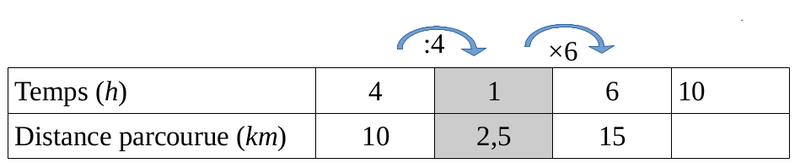
\includegraphics[scale=0.5]{tab3_2}
	\end{center}
\end{mymeth}

\subsubsection*{Avec le coefficient multiplicateur}

\begin{mymeth}
	On cherche par quel nombre on multiplie 4 pour obtenir 10. $4 \times ...= 10$.
	
	C’est le nombre \num{2.5} ($10 \div 4$). $6 \times \num{2.5} = 15$.
	
	
	\begin{center}
		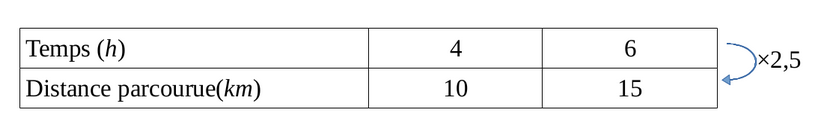
\includegraphics[scale=0.5]{tab3_3}
	\end{center}
\end{mymeth}


\subsubsection*{En utilisant les propriétés de la proportionnalité}

\begin{myprop}
	Dans un tableau de proportionnalité, on peut :
		\begin{itemize}
			\item multiplier/diviser une colonne par un nombre;
			\item ajouter/soustraire des colonnes entre elles.
		\end{itemize}
	
	\begin{center}
		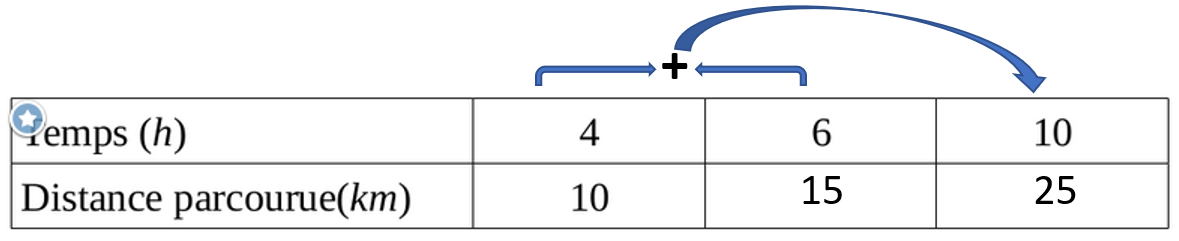
\includegraphics[scale=0.5]{tab3_4}
	\end{center}
\end{myprop}

\section{Pourcentages}

\subsection{Appliquer un pourcentage}

\begin{mydef}
	Un pourcentage traduit une situation de proportionnalité. 

	Un pourcentage est une proportion exprimée sur un total de 100 (de dénominateur égal à 100).
	
\end{mydef}

\begin{myex}
	<<Dans une confiture, il y a 60 \% de fruits>>
	\begin{itemize}
		\item La masse de fruits est proportionnelle à la masse totale de confiture.
		\item[$\Rightarrow$] Il y a 60g de fruits pour 100g de confiture.
	\end{itemize}
\end{myex}


\begin{myprop}
	$P$ est un nombre positif.
	
	Pour calculer $P\% $ d'une quantité, on multiplie cette quantité par $\frac{P}{100}$.
\end{myprop}


\begin{myex}
	Calculer $20 \% $ de 50 revient à multiplier 50 par $\frac{20}{100}$ :
	
	\begin{equation*}
		50 \times \dfrac{20}{100} = 50 \times \num{0.2} = 10
	\end{equation*}
	
	
	$20 \% $ de 50  vaut 10.
\end{myex}

\subsection{Calculer un taux de pourcentage}


\begin{myex}
	Dans un collège, il y a 800 élèves et 200 sont externes. Quel est le pourcentage d'externes ?\\
	
	
		\begin{tabular}{|l|l|l|}
			\hline
			Nombre d'externes & 200 & $P$ \\ \hline
			Nombre d'élèves   & 800 & 100 \\ \hline
		\end{tabular}
	
	\vspace*{0.5cm}

	
	Ce tableau est un tableau de proportionnalité. Le coefficient de proportionnalité est 4 ($800 \div 200$).
	
	Calcul de $P$ : $100 \div 4 = 25$.\\
	
	 Il y a $25 \%$ d'externes.
\end{myex}
\section{Notion d'échelle}

\begin{mydef}
	\begin{itemize}
		\item 	Sur un plan à \kw{l'échelle}, les longueurs sur le plan sont proportionnelles aux longueurs dans la réalité.
		
		\item  L'échelle d'un plan est  est le quotient de la longueur sur le plan par la longueur réelle correspondante, lorsque ces longueurs sont exprimées dans la même unité.
	\end{itemize}

\end{mydef}

\begin{myexs}
	\begin{enumerate}
		\item Un plan est à l'échelle $ 1 / \num{2000}$. Cela signifie que 1 cm sur le plan représente 20 m (\num{2000} cm) dans la réalité. Les longueurs du plan sont 2000 fois plus petites que les longueurs réelles.
		
		
		\item Un schéma est à l'échelle 50. Cela signifie que 1 cm sur le schéma représente \num{0.02} cm dans la réalité. Les longueurs du plan sont 50 fois plus grandes que les longueurs réelles.
		
		
		\item Sur une carte, 3 cm représentent  12 km dans la réalité. Quelle est l'échelle de la carte ?
		
		12 km = \num{1200000} cm.
		\begin{equation*}
		\dfrac{3}{\num{1200000}} = \dfrac{1}{\num{400000}}
		\end{equation*}
		
		L'échelle de cette carte est $1 / \num{400000}$.
	\end{enumerate}
\end{myexs}

\begin{myrems}
	\begin{itemize}
		\item Une échelle n'a pas d'unité.
		\item L'échelle d'un plan est est le nombre par lequel on multiplie les longueurs réelles pour obtenir les longueurs sur le plan, dans la même unité.
	\end{itemize}
\end{myrems}
\end{document}

